\documentclass[14pt]{article}
\usepackage{../../report-tex/styles}


\begin{document}

\titlewithlabnum{3}

\tableofcontents
\newpage

\section{Мета:}
Мета роботи – отримати вміння та навички використовувати інкапсуляцію, абстракцію типів, успадкування та поліморфізм на основі класів С++, запрограмувавши графічний інтерфейс користувача.
\section{Завдання:}
1. Створити у середовищі MS Visual Studio C++ проект Win32 з ім’ям Lab3.\\
2. Написати вихідний текст програми згідно варіанту завдання.\\
3. Скомпілювати вихідний текст і отримати виконуваний файл програми.\\
4. Перевірити роботу програми. Налагодити програму.\\
5. Проаналізувати та прокоментувати результати та вихідний текст програми.\\
6. Оформити звіт.\\

\subsection{Варіант: }
Варіанти завдань та основні вимоги\\
1. У звіті повинна бути схема успадкування класів – діаграма класів\\
2. Усі методи-обробники повідомлень, зокрема, і метод OnNotify, повинні бути функціями-членами деякого класу (класів).\\
3. Для вибору типу об’єкту в графічному редакторі Lab3 повинно бути вікно Toolbar з кнопками відповідно типам об'єктів. Кнопки дублюють підпункти меню "Об’єкти". Кнопки мають бути з підказками (tooltips). Меню "Об’єкти" повинно бути праворуч меню "Файл" та ліворуч меню "Довідка". Підпункти меню "Об’єкти" містять назви геометричних форм українською мовою. Геометричні форми згідно варіанту завдання.\\
4. Для вибору варіанту використовується значення Ж = Жлаб2 + 1, де\\
Жлаб2 – номер студента в журналі, який використовувався для попередньої лаб. роботи No2.\\

\begin{align}
    J &= 22 + 1 \\
    J &= 23
\end{align}
5. Масив вказівників для динамічних об’єктів типу Shape\\
- динамічний масив Shape **pcshape;\\
- статичний масив Shape *pcshape[N];\\
причому кількість елементів масиву вказівників як для статичного, так і динамічного має бути N = Ж+100. $ N = 23 + 100$\\
Динамічний масив обирають студенти, у яких варіант (Ж mod 3 = 0).\\
Решта студентів роблять статичний масив. Примітка. Позначка mod означає залишок від ділення. $ 23 \bmod 3 = 2$\\
6. "Гумовий" слід при вводі об’єктів\\
- суцільна лінія чорного кольору для варіантів (Ж mod 4 = 0)\\
- суцільна лінія червоного кольору для (Ж mod 4 = 1)\\
- суцільна лінія синього кольору для (Ж mod 4 = 2)\\
- пунктирна лінія чорного кольору для (Ж mod 4 =3) $ 23 \bmod 4 = 3$\\
7. Чотири геометричні форми (крапка, лінія, прямокутник, еліпс) можуть мати наступні різновиди вводу та відображення.\\
7.1. Прямокутник\\
Увід прямокутника:\\
- по двом протилежним кутам для варіантів (Ж mod 2 = 0)\\
- від центру до одного з кутів для (Ж mod 2 = 1) $ 23 \bmod 2 = 1$\\
Відображення прямокутника:\\
- чорний контур з білим заповненням для (Ж mod 5 = 0)\\
- чорний контур з кольоровим заповненням для (Ж mod 5 = 1 або 2)\\
- чорний контур прямокутника без заповнення для (Ж mod 5 = 3 або 4) $ 23 \bmod 5 = 3$\\
Кольори заповнення прямокутника:\\
- жовтий для (Ж mod 6 = 0)\\
- світло-зелений для (Ж mod 6 = 1)\\
- блакитний для (Ж mod 6 = 2)\\
- рожевий для (Ж mod 6 = 3)\\
- померанчевий для (Ж mod 6 = 4)\\
- сірий для (Ж mod 6 = 5) $ 23 \bmod 6 = 5$\\
7.2. Еліпс\\
Ввід еліпсу:\\
- по двом протилежним кутам охоплюючого прямокутника для варіантів (Ж mod 2 = 1) $ 23 \bmod 2 = 1 $\\
- від центру до одного з кутів охоплюючого прямокутника для варіантів (Ж mod 2 = 0)\\
Відображення еліпсу:\\
- чорний контур з білим заповненням для (Ж mod 5 = 1)\\
- чорний контур з кольоровим заповненням для (Ж mod 5 = 3 або 4) $ 23 \bmod 5 = 3$\\
- чорний контур еліпсу без заповнення для (Ж mod 5 = 0 або 2)\\
Кольори заповнення еліпсу:\\
- жовтий для (Ж mod 6 = 1)\\
- світло-зелений для (Ж mod 6 = 2)\\
- блакитний для (Ж mod 6 = 3)\\
- рожевий для (Ж mod 6 = 4)\\
- померанчевий для (Ж mod 6 = 5) $ 23 \bmod 6 = 5$\\
- сірий для (Ж mod 6 = 0)\\
8. Позначка поточного типу об’єкту, що вводиться\\
- в меню (метод OnInitMenuPopup) для варіантів (Ж mod 2 = 0)\\
- в заголовку вікна для (Ж mod 2 = 1) $ 23 \bmod 2 = 1$\\
Примітка. Визначення кольорів та інші параметри варіантів можуть бути змінені викладачем шляхом оголошення студентам відповідного повідомлення завчасно перед постановкою завдань.\\

\section{Текст програми:}
\subsection{Module: com.github.erotourtes.drawing.editor}
\lstinputlistingukr{DmProcessor.kt}{../src/main/kotlin/com/github/erotourtes/drawing/editor/DmProcessor.kt}
\lstinputlistingukr{Editor.kt}{../src/main/kotlin/com/github/erotourtes/drawing/editor/Editor.kt}
\lstinputlistingukr{Editors.kt}{../src/main/kotlin/com/github/erotourtes/drawing/editor/Editors.kt}
\lstinputlistingukr{ShapesList.kt}{../src/main/kotlin/com/github/erotourtes/drawing/editor/ShapesList.kt}

\subsection{Module: 1.0}
\lstinputlistingukr{MANIFEST.MF}{../src/main/resources/META-INF/MANIFEST.MF}

\subsection{Module: com.github.erotourtes.view}
\lstinputlistingukr{MainController.kt}{../src/main/kotlin/com/github/erotourtes/view/MainController.kt}
\lstinputlistingukr{MainView.kt}{../src/main/kotlin/com/github/erotourtes/view/MainView.kt}
\lstinputlistingukr{MenuBar.kt}{../src/main/kotlin/com/github/erotourtes/view/MenuBar.kt}
\lstinputlistingukr{ToolBar.kt}{../src/main/kotlin/com/github/erotourtes/view/ToolBar.kt}

\subsection{Module: com.github.erotourtes.app}
\lstinputlistingukr{MyApp.kt}{../src/main/kotlin/com/github/erotourtes/app/MyApp.kt}

\subsection{Module: com.github.erotourtes.drawing}
\lstinputlistingukr{CanvasPane.kt}{../src/main/kotlin/com/github/erotourtes/drawing/CanvasPane.kt}
\lstinputlistingukr{EditorHandler.kt}{../src/main/kotlin/com/github/erotourtes/drawing/EditorHandler.kt}

\subsection{Module: com.github.erotourtes.drawing.shape}
\lstinputlistingukr{Shape.kt}{../src/main/kotlin/com/github/erotourtes/drawing/shape/Shape.kt}
\lstinputlistingukr{Shapes.kt}{../src/main/kotlin/com/github/erotourtes/drawing/shape/Shapes.kt}

\subsection{Module: com.github.erotourtes.styles}
\lstinputlistingukr{ToolbarStyles.kt}{../src/main/kotlin/com/github/erotourtes/styles/ToolbarStyles.kt}

\subsection{Module: com.github.erotourtes.utils}
\lstinputlistingukr{Dimension.kt}{../src/main/kotlin/com/github/erotourtes/utils/Dimension.kt}
\lstinputlistingukr{ExtensionFunctions.kt}{../src/main/kotlin/com/github/erotourtes/utils/ExtensionFunctions.kt}
\lstinputlistingukr{Utils.kt}{../src/main/kotlin/com/github/erotourtes/utils/Utils.kt}



\section{Ілюстрації:}
\begin{figure}[H]
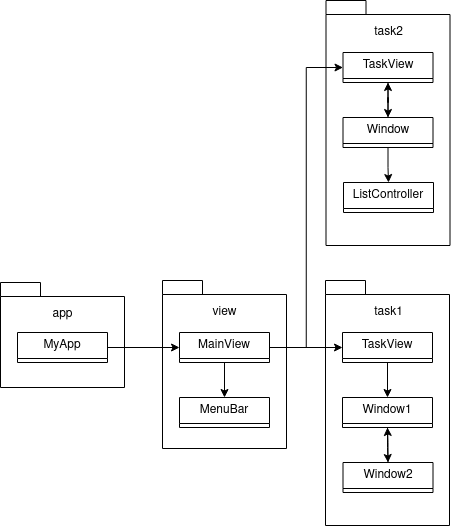
\includegraphics[width=10cm]{1}
\centering
\end{figure}


\section{Висновки:}
Отже, я отримав вміння та навички використовувати інкапсуляцію, абстракцію типів, успадкування та поліморфізм на основі класів Kotlin, запрограмувавши графічний інтерфейс користувача.
\end{document}
